\documentclass[twoside]{book}

% Packages required by doxygen
\usepackage{calc}
\usepackage{doxygen}
\usepackage{graphicx}
\usepackage[utf8]{inputenc}
\usepackage{makeidx}
\usepackage{multicol}
\usepackage{multirow}
\usepackage{fixltx2e}
\PassOptionsToPackage{warn}{textcomp}
\usepackage{textcomp}
\usepackage[nointegrals]{wasysym}
\usepackage[table]{xcolor}

% Font selection
\usepackage[T1]{fontenc}
\usepackage{mathptmx}
\usepackage[scaled=.90]{helvet}
\usepackage{courier}
\usepackage{amssymb}
\usepackage{sectsty}
\renewcommand{\familydefault}{\sfdefault}
\allsectionsfont{%
  \fontseries{bc}\selectfont%
  \color{darkgray}%
}
\renewcommand{\DoxyLabelFont}{%
  \fontseries{bc}\selectfont%
  \color{darkgray}%
}
\newcommand{\+}{\discretionary{\mbox{\scriptsize$\hookleftarrow$}}{}{}}

% Page & text layout
\usepackage{geometry}
\geometry{%
  a4paper,%
  top=2.5cm,%
  bottom=2.5cm,%
  left=2.5cm,%
  right=2.5cm%
}
\tolerance=750
\hfuzz=15pt
\hbadness=750
\setlength{\emergencystretch}{15pt}
\setlength{\parindent}{0cm}
\setlength{\parskip}{0.2cm}
\makeatletter
\renewcommand{\paragraph}{%
  \@startsection{paragraph}{4}{0ex}{-1.0ex}{1.0ex}{%
    \normalfont\normalsize\bfseries\SS@parafont%
  }%
}
\renewcommand{\subparagraph}{%
  \@startsection{subparagraph}{5}{0ex}{-1.0ex}{1.0ex}{%
    \normalfont\normalsize\bfseries\SS@subparafont%
  }%
}
\makeatother

% Headers & footers
\usepackage{fancyhdr}
\pagestyle{fancyplain}
\fancyhead[LE]{\fancyplain{}{\bfseries\thepage}}
\fancyhead[CE]{\fancyplain{}{}}
\fancyhead[RE]{\fancyplain{}{\bfseries\leftmark}}
\fancyhead[LO]{\fancyplain{}{\bfseries\rightmark}}
\fancyhead[CO]{\fancyplain{}{}}
\fancyhead[RO]{\fancyplain{}{\bfseries\thepage}}
\fancyfoot[LE]{\fancyplain{}{}}
\fancyfoot[CE]{\fancyplain{}{}}
\fancyfoot[RE]{\fancyplain{}{\bfseries\scriptsize Generated on Mon Jun 9 2014 10\+:08\+:22 for My Project by Doxygen }}
\fancyfoot[LO]{\fancyplain{}{\bfseries\scriptsize Generated on Mon Jun 9 2014 10\+:08\+:22 for My Project by Doxygen }}
\fancyfoot[CO]{\fancyplain{}{}}
\fancyfoot[RO]{\fancyplain{}{}}
\renewcommand{\footrulewidth}{0.4pt}
\renewcommand{\chaptermark}[1]{%
  \markboth{#1}{}%
}
\renewcommand{\sectionmark}[1]{%
  \markright{\thesection\ #1}%
}

% Indices & bibliography
\usepackage{natbib}
\usepackage[titles]{tocloft}
\setcounter{tocdepth}{3}
\setcounter{secnumdepth}{5}
\makeindex

% Hyperlinks (required, but should be loaded last)
\usepackage{ifpdf}
\ifpdf
  \usepackage[pdftex,pagebackref=true]{hyperref}
\else
  \usepackage[ps2pdf,pagebackref=true]{hyperref}
\fi
\hypersetup{%
  colorlinks=true,%
  linkcolor=blue,%
  citecolor=blue,%
  unicode%
}

% Custom commands
\newcommand{\clearemptydoublepage}{%
  \newpage{\pagestyle{empty}\cleardoublepage}%
}


%===== C O N T E N T S =====

\begin{document}

% Titlepage & ToC
\hypersetup{pageanchor=false,
             bookmarks=true,
             bookmarksnumbered=true,
             pdfencoding=unicode
            }
\pagenumbering{roman}
\begin{titlepage}
\vspace*{7cm}
\begin{center}%
{\Large My Project }\\
\vspace*{1cm}
{\large Generated by Doxygen 1.8.7}\\
\vspace*{0.5cm}
{\small Mon Jun 9 2014 10:08:22}\\
\end{center}
\end{titlepage}
\clearemptydoublepage
\tableofcontents
\clearemptydoublepage
\pagenumbering{arabic}
\hypersetup{pageanchor=true}

%--- Begin generated contents ---
\chapter{Hierarchical Index}
\section{Class Hierarchy}
This inheritance list is sorted roughly, but not completely, alphabetically\+:\begin{DoxyCompactList}
\item \contentsline{section}{Answers}{\pageref{class_answers}}{}
\item \contentsline{section}{item}{\pageref{classitem}}{}
\item \contentsline{section}{jugador}{\pageref{classjugador}}{}
\item \contentsline{section}{paciente}{\pageref{classpaciente}}{}
\item \contentsline{section}{Question}{\pageref{class_question}}{}
\begin{DoxyCompactList}
\item \contentsline{section}{question\+\_\+matriz}{\pageref{classquestion__matriz}}{}
\end{DoxyCompactList}
\item \contentsline{section}{resultado}{\pageref{classresultado}}{}
\end{DoxyCompactList}

\chapter{Class Index}
\section{Class List}
Here are the classes, structs, unions and interfaces with brief descriptions\+:\begin{DoxyCompactList}
\item\contentsline{section}{\hyperlink{class_answers}{Answers} }{\pageref{class_answers}}{}
\item\contentsline{section}{\hyperlink{classitem}{item} }{\pageref{classitem}}{}
\item\contentsline{section}{\hyperlink{classjugador}{jugador} }{\pageref{classjugador}}{}
\item\contentsline{section}{\hyperlink{classpaciente}{paciente} }{\pageref{classpaciente}}{}
\item\contentsline{section}{\hyperlink{class_question}{Question} }{\pageref{class_question}}{}
\item\contentsline{section}{\hyperlink{classquestion__matriz}{question\+\_\+matriz} }{\pageref{classquestion__matriz}}{}
\item\contentsline{section}{\hyperlink{classresultado}{resultado} }{\pageref{classresultado}}{}
\end{DoxyCompactList}

\chapter{File Index}
\section{File List}
Here is a list of all files with brief descriptions\+:\begin{DoxyCompactList}
\item\contentsline{section}{\hyperlink{_answers_8hpp}{Answers.\+hpp} }{\pageref{_answers_8hpp}}{}
\item\contentsline{section}{\hyperlink{_item_8hpp}{Item.\+hpp} }{\pageref{_item_8hpp}}{}
\item\contentsline{section}{\hyperlink{_jugador_8hpp}{Jugador.\+hpp} }{\pageref{_jugador_8hpp}}{}
\item\contentsline{section}{\hyperlink{paciente_8hpp}{paciente.\+hpp} }{\pageref{paciente_8hpp}}{}
\item\contentsline{section}{\hyperlink{_question_8hpp}{Question.\+hpp} }{\pageref{_question_8hpp}}{}
\item\contentsline{section}{\hyperlink{resultado_8hpp}{resultado.\+hpp} }{\pageref{resultado_8hpp}}{}
\item\contentsline{section}{J\+U\+E\+G\+O C\+S\+U4/\hyperlink{_complement_8hpp}{Complement.\+hpp} }{\pageref{_complement_8hpp}}{}
\item\contentsline{section}{J\+U\+E\+G\+O C\+S\+U4/\hyperlink{_pruebas_8cpp}{Pruebas.\+cpp} }{\pageref{_pruebas_8cpp}}{}
\item\contentsline{section}{J\+U\+E\+G\+O M\+E\+M\+O/\hyperlink{_complement2_8hpp}{Complement2.\+hpp} }{\pageref{_complement2_8hpp}}{}
\item\contentsline{section}{J\+U\+E\+G\+O M\+E\+M\+O/\hyperlink{_prueba2_8cpp}{Prueba2.\+cpp} }{\pageref{_prueba2_8cpp}}{}
\end{DoxyCompactList}

\chapter{Class Documentation}
\hypertarget{class_answers}{\section{Answers Class Reference}
\label{class_answers}\index{Answers@{Answers}}
}


{\ttfamily \#include $<$Answers.\+hpp$>$}

\subsection*{Public Member Functions}
\begin{DoxyCompactItemize}
\item 
\hyperlink{class_answers_a086ca4b89b92048a18a2f03a56bf939c}{Answers} ()
\item 
\hyperlink{class_answers_a50fed75a419899e378cb414a0feeafe5}{Answers} (int n)
\item 
\hyperlink{class_answers_aa68607fa9eca1dd77051508d3d19fd93}{Answers} (int n, int s)
\item 
void \hyperlink{class_answers_a319ff5a552ff021dc289fa977b4de285}{add\+\_\+ans} (int i)
\item 
vector$<$ int $>$ \hyperlink{class_answers_a7c634663a8832fc41c07fd70349d9e72}{get\+\_\+ans} ()
\item 
\hyperlink{class_answers_aab5e74ea364d110c732670da14a46d3d}{$\sim$\+Answers} ()
\begin{DoxyCompactList}\small\item\em Destructor. \end{DoxyCompactList}\end{DoxyCompactItemize}


\subsection{Detailed Description}
Answer is a class conformed by a vector$<$int$>$

This class is focused to be the answer of a question or the sellection is made by the user 

\subsection{Constructor \& Destructor Documentation}
\hypertarget{class_answers_a086ca4b89b92048a18a2f03a56bf939c}{\index{Answers@{Answers}!Answers@{Answers}}
\index{Answers@{Answers}!Answers@{Answers}}
\subsubsection[{Answers}]{\setlength{\rightskip}{0pt plus 5cm}Answers\+::\+Answers (
\begin{DoxyParamCaption}
{}
\end{DoxyParamCaption}
)\hspace{0.3cm}{\ttfamily [inline]}}}\label{class_answers_a086ca4b89b92048a18a2f03a56bf939c}
Constructor by default Creates an \hyperlink{class_answers}{Answers} type with default parameters  $<$none$>$ \begin{DoxySeeAlso}{See also}
\hyperlink{class_answers_a50fed75a419899e378cb414a0feeafe5}{Answers(int n)}, \hyperlink{class_answers_aa68607fa9eca1dd77051508d3d19fd93}{Answers(int n,int s)} 
\end{DoxySeeAlso}
\hypertarget{class_answers_a50fed75a419899e378cb414a0feeafe5}{\index{Answers@{Answers}!Answers@{Answers}}
\index{Answers@{Answers}!Answers@{Answers}}
\subsubsection[{Answers}]{\setlength{\rightskip}{0pt plus 5cm}Answers\+::\+Answers (
\begin{DoxyParamCaption}
\item[{int}]{n}
\end{DoxyParamCaption}
)\hspace{0.3cm}{\ttfamily [inline]}}}\label{class_answers_a50fed75a419899e378cb414a0feeafe5}
Constructor depending on an integer Create an \hyperlink{class_answers}{Answers} type with \char`\"{}n\char`\"{} integers where the user decides what value will get each integer. 
\begin{DoxyParams}{Parameters}
{\em n} & an integer argument \\
\hline
\end{DoxyParams}
\begin{DoxySeeAlso}{See also}
\hyperlink{class_answers_a086ca4b89b92048a18a2f03a56bf939c}{Answers()}, \hyperlink{class_answers_aa68607fa9eca1dd77051508d3d19fd93}{Answers(int n,int s)} 
\end{DoxySeeAlso}
\hypertarget{class_answers_aa68607fa9eca1dd77051508d3d19fd93}{\index{Answers@{Answers}!Answers@{Answers}}
\index{Answers@{Answers}!Answers@{Answers}}
\subsubsection[{Answers}]{\setlength{\rightskip}{0pt plus 5cm}Answers\+::\+Answers (
\begin{DoxyParamCaption}
\item[{int}]{n, }
\item[{int}]{s}
\end{DoxyParamCaption}
)\hspace{0.3cm}{\ttfamily [inline]}}}\label{class_answers_aa68607fa9eca1dd77051508d3d19fd93}
Constructor depending on an integer Create an \hyperlink{class_answers}{Answers} type with \char`\"{}n\char`\"{} integers where each one 
\begin{DoxyParams}{Parameters}
{\em n} & an integer argument \\
\hline
{\em s} & an integer argument \\
\hline
\end{DoxyParams}
\begin{DoxySeeAlso}{See also}
\hyperlink{class_answers_a086ca4b89b92048a18a2f03a56bf939c}{Answers()}, \hyperlink{class_answers_a50fed75a419899e378cb414a0feeafe5}{Answers(int n)} 
\end{DoxySeeAlso}
\hypertarget{class_answers_aab5e74ea364d110c732670da14a46d3d}{\index{Answers@{Answers}!````~Answers@{$\sim$\+Answers}}
\index{````~Answers@{$\sim$\+Answers}!Answers@{Answers}}
\subsubsection[{$\sim$\+Answers}]{\setlength{\rightskip}{0pt plus 5cm}Answers\+::$\sim$\+Answers (
\begin{DoxyParamCaption}
{}
\end{DoxyParamCaption}
)\hspace{0.3cm}{\ttfamily [inline]}}}\label{class_answers_aab5e74ea364d110c732670da14a46d3d}


Destructor. 

Destroys the \hyperlink{class_answers}{Answers} type. 

\subsection{Member Function Documentation}
\hypertarget{class_answers_a319ff5a552ff021dc289fa977b4de285}{\index{Answers@{Answers}!add\+\_\+ans@{add\+\_\+ans}}
\index{add\+\_\+ans@{add\+\_\+ans}!Answers@{Answers}}
\subsubsection[{add\+\_\+ans}]{\setlength{\rightskip}{0pt plus 5cm}void Answers\+::add\+\_\+ans (
\begin{DoxyParamCaption}
\item[{int}]{i}
\end{DoxyParamCaption}
)\hspace{0.3cm}{\ttfamily [inline]}}}\label{class_answers_a319ff5a552ff021dc289fa977b4de285}
\hypertarget{class_answers_a7c634663a8832fc41c07fd70349d9e72}{\index{Answers@{Answers}!get\+\_\+ans@{get\+\_\+ans}}
\index{get\+\_\+ans@{get\+\_\+ans}!Answers@{Answers}}
\subsubsection[{get\+\_\+ans}]{\setlength{\rightskip}{0pt plus 5cm}vector$<$int$>$ Answers\+::get\+\_\+ans (
\begin{DoxyParamCaption}
{}
\end{DoxyParamCaption}
)\hspace{0.3cm}{\ttfamily [inline]}}}\label{class_answers_a7c634663a8832fc41c07fd70349d9e72}


The documentation for this class was generated from the following file\+:\begin{DoxyCompactItemize}
\item 
\hyperlink{_answers_8hpp}{Answers.\+hpp}\end{DoxyCompactItemize}

\hypertarget{classitem}{\section{item Class Reference}
\label{classitem}\index{item@{item}}
}


{\ttfamily \#include $<$Item.\+hpp$>$}

\subsection*{Public Member Functions}
\begin{DoxyCompactItemize}
\item 
\hyperlink{classitem_a344fbf6e3db0d59e0c8ac75cd42ee144}{item} ()
\item 
void \hyperlink{classitem_a2ffe516ed0acc8638af2d743fce0cbb0}{Set\+\_\+value} (int id)
\item 
\hyperlink{classitem_ac8395f04ecf257cd8a80e15f8ceb53fe}{item} (int s)
\item 
int \hyperlink{classitem_a7ceb113f8aa1662fbf74b53714d65da7}{get\+\_\+value} ()
\item 
\hyperlink{classitem_ae1792174ea9d664d6413f5ad0de38d74}{$\sim$item} ()
\end{DoxyCompactItemize}


\subsection{Constructor \& Destructor Documentation}
\hypertarget{classitem_a344fbf6e3db0d59e0c8ac75cd42ee144}{\index{item@{item}!item@{item}}
\index{item@{item}!item@{item}}
\subsubsection[{item}]{\setlength{\rightskip}{0pt plus 5cm}item\+::item (
\begin{DoxyParamCaption}
{}
\end{DoxyParamCaption}
)\hspace{0.3cm}{\ttfamily [inline]}}}\label{classitem_a344fbf6e3db0d59e0c8ac75cd42ee144}
\hypertarget{classitem_ac8395f04ecf257cd8a80e15f8ceb53fe}{\index{item@{item}!item@{item}}
\index{item@{item}!item@{item}}
\subsubsection[{item}]{\setlength{\rightskip}{0pt plus 5cm}item\+::item (
\begin{DoxyParamCaption}
\item[{int}]{s}
\end{DoxyParamCaption}
)\hspace{0.3cm}{\ttfamily [inline]}}}\label{classitem_ac8395f04ecf257cd8a80e15f8ceb53fe}
\hypertarget{classitem_ae1792174ea9d664d6413f5ad0de38d74}{\index{item@{item}!````~item@{$\sim$item}}
\index{````~item@{$\sim$item}!item@{item}}
\subsubsection[{$\sim$item}]{\setlength{\rightskip}{0pt plus 5cm}item\+::$\sim$item (
\begin{DoxyParamCaption}
{}
\end{DoxyParamCaption}
)\hspace{0.3cm}{\ttfamily [inline]}}}\label{classitem_ae1792174ea9d664d6413f5ad0de38d74}


\subsection{Member Function Documentation}
\hypertarget{classitem_a7ceb113f8aa1662fbf74b53714d65da7}{\index{item@{item}!get\+\_\+value@{get\+\_\+value}}
\index{get\+\_\+value@{get\+\_\+value}!item@{item}}
\subsubsection[{get\+\_\+value}]{\setlength{\rightskip}{0pt plus 5cm}int item\+::get\+\_\+value (
\begin{DoxyParamCaption}
{}
\end{DoxyParamCaption}
)\hspace{0.3cm}{\ttfamily [inline]}}}\label{classitem_a7ceb113f8aa1662fbf74b53714d65da7}
\hypertarget{classitem_a2ffe516ed0acc8638af2d743fce0cbb0}{\index{item@{item}!Set\+\_\+value@{Set\+\_\+value}}
\index{Set\+\_\+value@{Set\+\_\+value}!item@{item}}
\subsubsection[{Set\+\_\+value}]{\setlength{\rightskip}{0pt plus 5cm}void item\+::\+Set\+\_\+value (
\begin{DoxyParamCaption}
\item[{int}]{id}
\end{DoxyParamCaption}
)\hspace{0.3cm}{\ttfamily [inline]}}}\label{classitem_a2ffe516ed0acc8638af2d743fce0cbb0}


The documentation for this class was generated from the following file\+:\begin{DoxyCompactItemize}
\item 
\hyperlink{_item_8hpp}{Item.\+hpp}\end{DoxyCompactItemize}

\hypertarget{classjugador}{\section{jugador Class Reference}
\label{classjugador}\index{jugador@{jugador}}
}


{\ttfamily \#include $<$Jugador.\+hpp$>$}



The documentation for this class was generated from the following file\+:\begin{DoxyCompactItemize}
\item 
\hyperlink{_jugador_8hpp}{Jugador.\+hpp}\end{DoxyCompactItemize}

\hypertarget{classpaciente}{\section{paciente Class Reference}
\label{classpaciente}\index{paciente@{paciente}}
}


{\ttfamily \#include $<$paciente.\+hpp$>$}

\subsection*{Public Member Functions}
\begin{DoxyCompactItemize}
\item 
\hyperlink{classpaciente_afb82928ff5b28603dba5efe4c85b7462}{paciente} (std\+::string name, int cd, int age)
\item 
std\+::string \hyperlink{classpaciente_a6cddb865d694a11ed08610b88432a727}{get\+\_\+name} ()
\item 
int \hyperlink{classpaciente_afbf0e737dcf484dddc855d4374b29e46}{get\+\_\+codigo} ()
\item 
int \hyperlink{classpaciente_ae3b3a231110550f58fb7acef4a1f2740}{get\+\_\+edad} ()
\end{DoxyCompactItemize}


\subsection{Constructor \& Destructor Documentation}
\hypertarget{classpaciente_afb82928ff5b28603dba5efe4c85b7462}{\index{paciente@{paciente}!paciente@{paciente}}
\index{paciente@{paciente}!paciente@{paciente}}
\subsubsection[{paciente}]{\setlength{\rightskip}{0pt plus 5cm}paciente\+::paciente (
\begin{DoxyParamCaption}
\item[{std\+::string}]{name, }
\item[{int}]{cd, }
\item[{int}]{age}
\end{DoxyParamCaption}
)\hspace{0.3cm}{\ttfamily [inline]}}}\label{classpaciente_afb82928ff5b28603dba5efe4c85b7462}


\subsection{Member Function Documentation}
\hypertarget{classpaciente_afbf0e737dcf484dddc855d4374b29e46}{\index{paciente@{paciente}!get\+\_\+codigo@{get\+\_\+codigo}}
\index{get\+\_\+codigo@{get\+\_\+codigo}!paciente@{paciente}}
\subsubsection[{get\+\_\+codigo}]{\setlength{\rightskip}{0pt plus 5cm}int paciente\+::get\+\_\+codigo (
\begin{DoxyParamCaption}
{}
\end{DoxyParamCaption}
)\hspace{0.3cm}{\ttfamily [inline]}}}\label{classpaciente_afbf0e737dcf484dddc855d4374b29e46}
\hypertarget{classpaciente_ae3b3a231110550f58fb7acef4a1f2740}{\index{paciente@{paciente}!get\+\_\+edad@{get\+\_\+edad}}
\index{get\+\_\+edad@{get\+\_\+edad}!paciente@{paciente}}
\subsubsection[{get\+\_\+edad}]{\setlength{\rightskip}{0pt plus 5cm}int paciente\+::get\+\_\+edad (
\begin{DoxyParamCaption}
{}
\end{DoxyParamCaption}
)\hspace{0.3cm}{\ttfamily [inline]}}}\label{classpaciente_ae3b3a231110550f58fb7acef4a1f2740}
\hypertarget{classpaciente_a6cddb865d694a11ed08610b88432a727}{\index{paciente@{paciente}!get\+\_\+name@{get\+\_\+name}}
\index{get\+\_\+name@{get\+\_\+name}!paciente@{paciente}}
\subsubsection[{get\+\_\+name}]{\setlength{\rightskip}{0pt plus 5cm}std\+::string paciente\+::get\+\_\+name (
\begin{DoxyParamCaption}
{}
\end{DoxyParamCaption}
)\hspace{0.3cm}{\ttfamily [inline]}}}\label{classpaciente_a6cddb865d694a11ed08610b88432a727}


The documentation for this class was generated from the following file\+:\begin{DoxyCompactItemize}
\item 
\hyperlink{paciente_8hpp}{paciente.\+hpp}\end{DoxyCompactItemize}

\hypertarget{class_question}{\section{Question Class Reference}
\label{class_question}\index{Question@{Question}}
}


{\ttfamily \#include $<$Question.\+hpp$>$}

Inheritance diagram for Question\+:\begin{figure}[H]
\begin{center}
\leavevmode
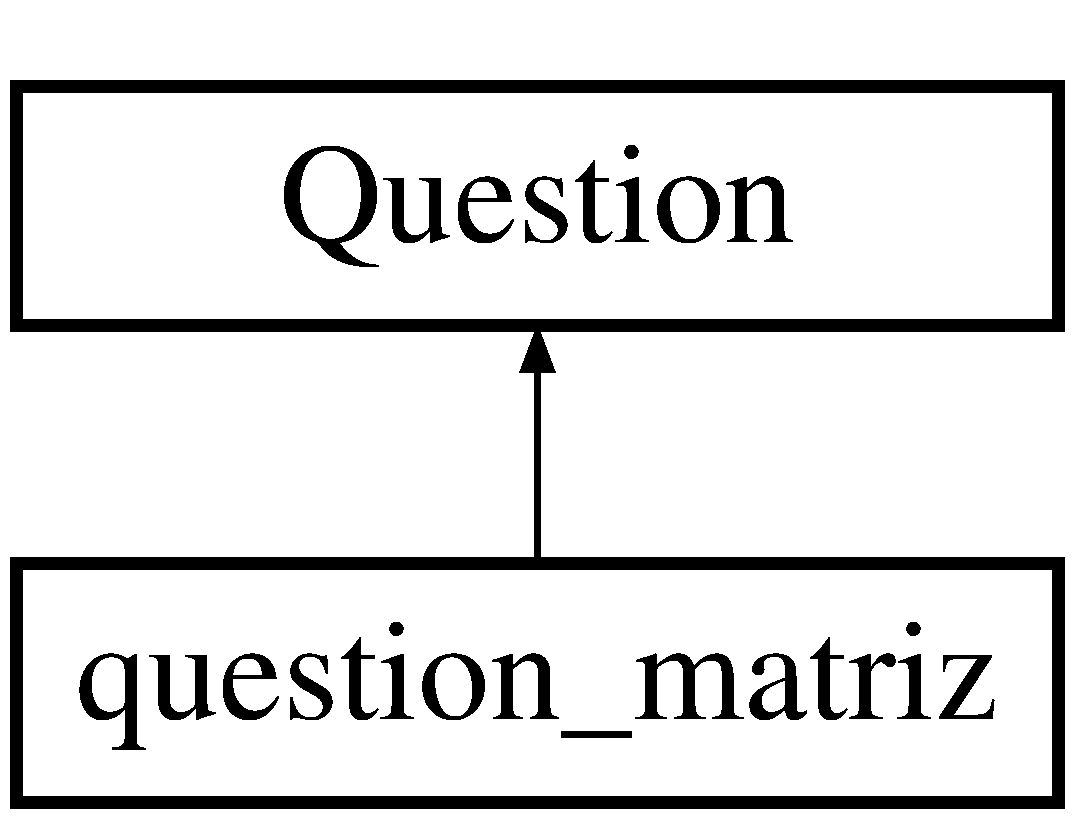
\includegraphics[height=2.000000cm]{class_question}
\end{center}
\end{figure}
\subsection*{Public Member Functions}
\begin{DoxyCompactItemize}
\item 
\hyperlink{class_question_a2e1167d0407c7530b4f7a7492d0050d0}{Question} ()
\item 
\hyperlink{class_question_a958c203567c631b25004074f478d205b}{Question} (int n, int s)
\item 
void \hyperlink{class_question_a7b457f4106d45132ad45d22ad621f3f9}{Set\+\_\+level} (int l)
\item 
void \hyperlink{class_question_a0bb8e8be70b5ccc72e9918bca35ca35a}{add\+\_\+item} (int n)
\item 
vector$<$ \hyperlink{classitem}{item} $>$ \hyperlink{class_question_afafe6fd5ed376966f808c65749da510a}{get\+\_\+\+Object} ()
\item 
vector$<$ int $>$ \hyperlink{class_question_aa0a8d162db42d785f5050634a4dc9471}{Show\+\_\+question\+\_\+val} ()
\item 
\hyperlink{class_question_a8d9283fb5357e39ed58a743f18629040}{$\sim$\+Question} ()
\end{DoxyCompactItemize}
\subsection*{Protected Attributes}
\begin{DoxyCompactItemize}
\item 
vector$<$ \hyperlink{classitem}{item} $>$ \hyperlink{class_question_aee4dca57403e91e0f2062499ba2955a9}{Objetos}
\end{DoxyCompactItemize}


\subsection{Constructor \& Destructor Documentation}
\hypertarget{class_question_a2e1167d0407c7530b4f7a7492d0050d0}{\index{Question@{Question}!Question@{Question}}
\index{Question@{Question}!Question@{Question}}
\subsubsection[{Question}]{\setlength{\rightskip}{0pt plus 5cm}Question\+::\+Question (
\begin{DoxyParamCaption}
{}
\end{DoxyParamCaption}
)\hspace{0.3cm}{\ttfamily [inline]}}}\label{class_question_a2e1167d0407c7530b4f7a7492d0050d0}
\hypertarget{class_question_a958c203567c631b25004074f478d205b}{\index{Question@{Question}!Question@{Question}}
\index{Question@{Question}!Question@{Question}}
\subsubsection[{Question}]{\setlength{\rightskip}{0pt plus 5cm}Question\+::\+Question (
\begin{DoxyParamCaption}
\item[{int}]{n, }
\item[{int}]{s}
\end{DoxyParamCaption}
)\hspace{0.3cm}{\ttfamily [inline]}}}\label{class_question_a958c203567c631b25004074f478d205b}
\hypertarget{class_question_a8d9283fb5357e39ed58a743f18629040}{\index{Question@{Question}!````~Question@{$\sim$\+Question}}
\index{````~Question@{$\sim$\+Question}!Question@{Question}}
\subsubsection[{$\sim$\+Question}]{\setlength{\rightskip}{0pt plus 5cm}Question\+::$\sim$\+Question (
\begin{DoxyParamCaption}
{}
\end{DoxyParamCaption}
)\hspace{0.3cm}{\ttfamily [inline]}}}\label{class_question_a8d9283fb5357e39ed58a743f18629040}


\subsection{Member Function Documentation}
\hypertarget{class_question_a0bb8e8be70b5ccc72e9918bca35ca35a}{\index{Question@{Question}!add\+\_\+item@{add\+\_\+item}}
\index{add\+\_\+item@{add\+\_\+item}!Question@{Question}}
\subsubsection[{add\+\_\+item}]{\setlength{\rightskip}{0pt plus 5cm}void Question\+::add\+\_\+item (
\begin{DoxyParamCaption}
\item[{int}]{n}
\end{DoxyParamCaption}
)\hspace{0.3cm}{\ttfamily [inline]}}}\label{class_question_a0bb8e8be70b5ccc72e9918bca35ca35a}
\hypertarget{class_question_afafe6fd5ed376966f808c65749da510a}{\index{Question@{Question}!get\+\_\+\+Object@{get\+\_\+\+Object}}
\index{get\+\_\+\+Object@{get\+\_\+\+Object}!Question@{Question}}
\subsubsection[{get\+\_\+\+Object}]{\setlength{\rightskip}{0pt plus 5cm}vector$<${\bf item}$>$ Question\+::get\+\_\+\+Object (
\begin{DoxyParamCaption}
{}
\end{DoxyParamCaption}
)\hspace{0.3cm}{\ttfamily [inline]}}}\label{class_question_afafe6fd5ed376966f808c65749da510a}
\hypertarget{class_question_a7b457f4106d45132ad45d22ad621f3f9}{\index{Question@{Question}!Set\+\_\+level@{Set\+\_\+level}}
\index{Set\+\_\+level@{Set\+\_\+level}!Question@{Question}}
\subsubsection[{Set\+\_\+level}]{\setlength{\rightskip}{0pt plus 5cm}void Question\+::\+Set\+\_\+level (
\begin{DoxyParamCaption}
\item[{int}]{l}
\end{DoxyParamCaption}
)\hspace{0.3cm}{\ttfamily [inline]}}}\label{class_question_a7b457f4106d45132ad45d22ad621f3f9}
\hypertarget{class_question_aa0a8d162db42d785f5050634a4dc9471}{\index{Question@{Question}!Show\+\_\+question\+\_\+val@{Show\+\_\+question\+\_\+val}}
\index{Show\+\_\+question\+\_\+val@{Show\+\_\+question\+\_\+val}!Question@{Question}}
\subsubsection[{Show\+\_\+question\+\_\+val}]{\setlength{\rightskip}{0pt plus 5cm}vector$<$int$>$ Question\+::\+Show\+\_\+question\+\_\+val (
\begin{DoxyParamCaption}
{}
\end{DoxyParamCaption}
)\hspace{0.3cm}{\ttfamily [inline]}}}\label{class_question_aa0a8d162db42d785f5050634a4dc9471}


\subsection{Member Data Documentation}
\hypertarget{class_question_aee4dca57403e91e0f2062499ba2955a9}{\index{Question@{Question}!Objetos@{Objetos}}
\index{Objetos@{Objetos}!Question@{Question}}
\subsubsection[{Objetos}]{\setlength{\rightskip}{0pt plus 5cm}vector$<${\bf item}$>$ Question\+::\+Objetos\hspace{0.3cm}{\ttfamily [protected]}}}\label{class_question_aee4dca57403e91e0f2062499ba2955a9}


The documentation for this class was generated from the following file\+:\begin{DoxyCompactItemize}
\item 
\hyperlink{_question_8hpp}{Question.\+hpp}\end{DoxyCompactItemize}

\hypertarget{classquestion__matriz}{\section{question\+\_\+matriz Class Reference}
\label{classquestion__matriz}\index{question\+\_\+matriz@{question\+\_\+matriz}}
}


{\ttfamily \#include $<$Complement2.\+hpp$>$}

Inheritance diagram for question\+\_\+matriz\+:\begin{figure}[H]
\begin{center}
\leavevmode
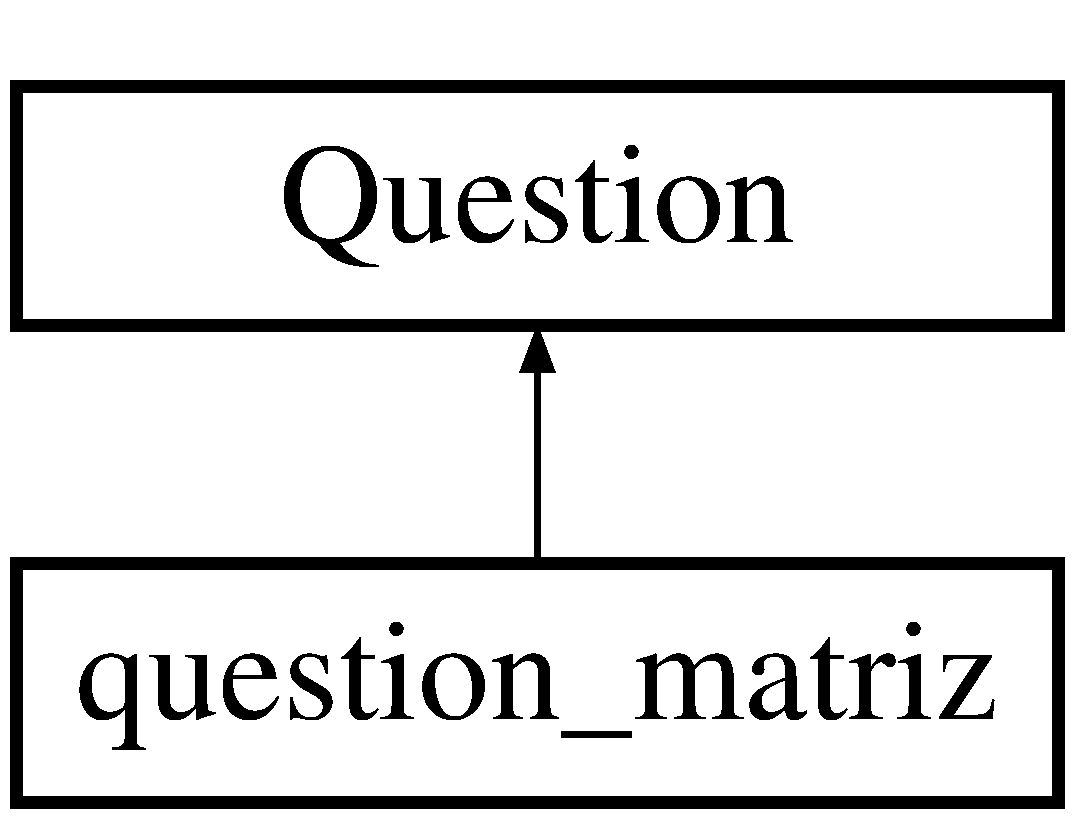
\includegraphics[height=2.000000cm]{classquestion__matriz}
\end{center}
\end{figure}
\subsection*{Public Member Functions}
\begin{DoxyCompactItemize}
\item 
\hyperlink{classquestion__matriz_ae3da8a30e2d7c23a4ca4cc59966f6bc7}{question\+\_\+matriz} ()
\item 
\hyperlink{classquestion__matriz_a8bbc3dc985d29946cad67cf328835714}{question\+\_\+matriz} (int n, int s)
\item 
void \hyperlink{classquestion__matriz_a1b6543dc9f0ff36cf44ccb47a141ca99}{show} (vector$<$ \hyperlink{classitem}{item} $>$ lista, int n)
\item 
\hyperlink{classquestion__matriz_a4f6443c7deab499e22cc820fab59d705}{$\sim$question\+\_\+matriz} ()
\end{DoxyCompactItemize}
\subsection*{Additional Inherited Members}


\subsection{Constructor \& Destructor Documentation}
\hypertarget{classquestion__matriz_ae3da8a30e2d7c23a4ca4cc59966f6bc7}{\index{question\+\_\+matriz@{question\+\_\+matriz}!question\+\_\+matriz@{question\+\_\+matriz}}
\index{question\+\_\+matriz@{question\+\_\+matriz}!question\+\_\+matriz@{question\+\_\+matriz}}
\subsubsection[{question\+\_\+matriz}]{\setlength{\rightskip}{0pt plus 5cm}question\+\_\+matriz\+::question\+\_\+matriz (
\begin{DoxyParamCaption}
{}
\end{DoxyParamCaption}
)\hspace{0.3cm}{\ttfamily [inline]}}}\label{classquestion__matriz_ae3da8a30e2d7c23a4ca4cc59966f6bc7}
\hypertarget{classquestion__matriz_a8bbc3dc985d29946cad67cf328835714}{\index{question\+\_\+matriz@{question\+\_\+matriz}!question\+\_\+matriz@{question\+\_\+matriz}}
\index{question\+\_\+matriz@{question\+\_\+matriz}!question\+\_\+matriz@{question\+\_\+matriz}}
\subsubsection[{question\+\_\+matriz}]{\setlength{\rightskip}{0pt plus 5cm}question\+\_\+matriz\+::question\+\_\+matriz (
\begin{DoxyParamCaption}
\item[{int}]{n, }
\item[{int}]{s}
\end{DoxyParamCaption}
)\hspace{0.3cm}{\ttfamily [inline]}}}\label{classquestion__matriz_a8bbc3dc985d29946cad67cf328835714}
\hypertarget{classquestion__matriz_a4f6443c7deab499e22cc820fab59d705}{\index{question\+\_\+matriz@{question\+\_\+matriz}!````~question\+\_\+matriz@{$\sim$question\+\_\+matriz}}
\index{````~question\+\_\+matriz@{$\sim$question\+\_\+matriz}!question\+\_\+matriz@{question\+\_\+matriz}}
\subsubsection[{$\sim$question\+\_\+matriz}]{\setlength{\rightskip}{0pt plus 5cm}question\+\_\+matriz\+::$\sim$question\+\_\+matriz (
\begin{DoxyParamCaption}
{}
\end{DoxyParamCaption}
)\hspace{0.3cm}{\ttfamily [inline]}}}\label{classquestion__matriz_a4f6443c7deab499e22cc820fab59d705}


\subsection{Member Function Documentation}
\hypertarget{classquestion__matriz_a1b6543dc9f0ff36cf44ccb47a141ca99}{\index{question\+\_\+matriz@{question\+\_\+matriz}!show@{show}}
\index{show@{show}!question\+\_\+matriz@{question\+\_\+matriz}}
\subsubsection[{show}]{\setlength{\rightskip}{0pt plus 5cm}void question\+\_\+matriz\+::show (
\begin{DoxyParamCaption}
\item[{vector$<$ {\bf item} $>$}]{lista, }
\item[{int}]{n}
\end{DoxyParamCaption}
)\hspace{0.3cm}{\ttfamily [inline]}}}\label{classquestion__matriz_a1b6543dc9f0ff36cf44ccb47a141ca99}


The documentation for this class was generated from the following file\+:\begin{DoxyCompactItemize}
\item 
J\+U\+E\+G\+O M\+E\+M\+O/\hyperlink{_complement2_8hpp}{Complement2.\+hpp}\end{DoxyCompactItemize}

\hypertarget{classresultado}{\section{resultado Class Reference}
\label{classresultado}\index{resultado@{resultado}}
}


{\ttfamily \#include $<$resultado.\+hpp$>$}

\subsection*{Public Member Functions}
\begin{DoxyCompactItemize}
\item 
\hyperlink{classresultado_ad79e4a65b2eb8370d62033222e4871e1}{resultado} (int t, int p)
\item 
int \hyperlink{classresultado_a61d5d1f185d9878e13444641e87cb3d5}{get\+\_\+tiempo} ()
\item 
int \hyperlink{classresultado_a3a8d4d428653c583ff5d914946b0c0a0}{get\+\_\+puntaje} ()
\end{DoxyCompactItemize}


\subsection{Constructor \& Destructor Documentation}
\hypertarget{classresultado_ad79e4a65b2eb8370d62033222e4871e1}{\index{resultado@{resultado}!resultado@{resultado}}
\index{resultado@{resultado}!resultado@{resultado}}
\subsubsection[{resultado}]{\setlength{\rightskip}{0pt plus 5cm}resultado\+::resultado (
\begin{DoxyParamCaption}
\item[{int}]{t, }
\item[{int}]{p}
\end{DoxyParamCaption}
)\hspace{0.3cm}{\ttfamily [inline]}}}\label{classresultado_ad79e4a65b2eb8370d62033222e4871e1}


\subsection{Member Function Documentation}
\hypertarget{classresultado_a3a8d4d428653c583ff5d914946b0c0a0}{\index{resultado@{resultado}!get\+\_\+puntaje@{get\+\_\+puntaje}}
\index{get\+\_\+puntaje@{get\+\_\+puntaje}!resultado@{resultado}}
\subsubsection[{get\+\_\+puntaje}]{\setlength{\rightskip}{0pt plus 5cm}int resultado\+::get\+\_\+puntaje (
\begin{DoxyParamCaption}
{}
\end{DoxyParamCaption}
)\hspace{0.3cm}{\ttfamily [inline]}}}\label{classresultado_a3a8d4d428653c583ff5d914946b0c0a0}
\hypertarget{classresultado_a61d5d1f185d9878e13444641e87cb3d5}{\index{resultado@{resultado}!get\+\_\+tiempo@{get\+\_\+tiempo}}
\index{get\+\_\+tiempo@{get\+\_\+tiempo}!resultado@{resultado}}
\subsubsection[{get\+\_\+tiempo}]{\setlength{\rightskip}{0pt plus 5cm}int resultado\+::get\+\_\+tiempo (
\begin{DoxyParamCaption}
{}
\end{DoxyParamCaption}
)\hspace{0.3cm}{\ttfamily [inline]}}}\label{classresultado_a61d5d1f185d9878e13444641e87cb3d5}


The documentation for this class was generated from the following file\+:\begin{DoxyCompactItemize}
\item 
\hyperlink{resultado_8hpp}{resultado.\+hpp}\end{DoxyCompactItemize}

\chapter{File Documentation}
\hypertarget{_answers_8hpp}{\section{Answers.\+hpp File Reference}
\label{_answers_8hpp}\index{Answers.\+hpp@{Answers.\+hpp}}
}
{\ttfamily \#include \char`\"{}item.\+hpp\char`\"{}}\\*
\subsection*{Classes}
\begin{DoxyCompactItemize}
\item 
class \hyperlink{class_answers}{Answers}
\end{DoxyCompactItemize}

\hypertarget{_item_8hpp}{\section{Item.\+hpp File Reference}
\label{_item_8hpp}\index{Item.\+hpp@{Item.\+hpp}}
}
{\ttfamily \#include $<$iostream$>$}\\*
{\ttfamily \#include $<$vector$>$}\\*
{\ttfamily \#include $<$list$>$}\\*
{\ttfamily \#include $<$string.\+h$>$}\\*
{\ttfamily \#include $<$cstdio$>$}\\*
{\ttfamily \#include $<$stdlib.\+h$>$}\\*
{\ttfamily \#include $<$time.\+h$>$}\\*
{\ttfamily \#include $<$iterator$>$}\\*
\subsection*{Classes}
\begin{DoxyCompactItemize}
\item 
class \hyperlink{classitem}{item}
\end{DoxyCompactItemize}

\hypertarget{_complement_8hpp}{\section{J\+U\+E\+G\+O C\+S\+U4/\+Complement.hpp File Reference}
\label{_complement_8hpp}\index{J\+U\+E\+G\+O C\+S\+U4/\+Complement.\+hpp@{J\+U\+E\+G\+O C\+S\+U4/\+Complement.\+hpp}}
}
{\ttfamily \#include \char`\"{}../item.\+hpp\char`\"{}}\\*
{\ttfamily \#include \char`\"{}../\+Question.\+hpp\char`\"{}}\\*
{\ttfamily \#include \char`\"{}../\+Answers.\+hpp\char`\"{}}\\*
\subsection*{Functions}
\begin{DoxyCompactItemize}
\item 
void \hyperlink{_complement_8hpp_a8254485fa2c2de8c13c433da84051d06}{printmat} (vector$<$ int $>$ lista, int n)
\item 
void \hyperlink{_complement_8hpp_adba7c84f980d4aac6ffb5095b21ea1c2}{print} (vector$<$ int $>$ lista)
\item 
void \hyperlink{_complement_8hpp_ab8405247118baa8e5f3c92f265aae620}{print} (vector$<$ \hyperlink{classitem}{item} $>$ lista)
\item 
int \hyperlink{_complement_8hpp_a08976a7d74874c7f4270900b29d1369b}{comparator} (vector$<$ int $>$ ans, vector$<$ \hyperlink{classitem}{item} $>$ ques)
\item 
vector$<$ int $>$ \hyperlink{_complement_8hpp_adf03879e40aeef0b654b2ce3797e845b}{comparator2} (vector$<$ int $>$ a, vector$<$ \hyperlink{classitem}{item} $>$ b)
\item 
int \hyperlink{_complement_8hpp_ab27432a461c59b93772baf60497382ba}{Juego} (vector$<$ \hyperlink{classitem}{item} $>$ b, int n)
\end{DoxyCompactItemize}


\subsection{Function Documentation}
\hypertarget{_complement_8hpp_a08976a7d74874c7f4270900b29d1369b}{\index{Complement.\+hpp@{Complement.\+hpp}!comparator@{comparator}}
\index{comparator@{comparator}!Complement.\+hpp@{Complement.\+hpp}}
\subsubsection[{comparator}]{\setlength{\rightskip}{0pt plus 5cm}int comparator (
\begin{DoxyParamCaption}
\item[{vector$<$ int $>$}]{ans, }
\item[{vector$<$ {\bf item} $>$}]{ques}
\end{DoxyParamCaption}
)}}\label{_complement_8hpp_a08976a7d74874c7f4270900b29d1369b}
\hypertarget{_complement_8hpp_adf03879e40aeef0b654b2ce3797e845b}{\index{Complement.\+hpp@{Complement.\+hpp}!comparator2@{comparator2}}
\index{comparator2@{comparator2}!Complement.\+hpp@{Complement.\+hpp}}
\subsubsection[{comparator2}]{\setlength{\rightskip}{0pt plus 5cm}vector$<$int$>$ comparator2 (
\begin{DoxyParamCaption}
\item[{vector$<$ int $>$}]{a, }
\item[{vector$<$ {\bf item} $>$}]{b}
\end{DoxyParamCaption}
)}}\label{_complement_8hpp_adf03879e40aeef0b654b2ce3797e845b}
\hypertarget{_complement_8hpp_ab27432a461c59b93772baf60497382ba}{\index{Complement.\+hpp@{Complement.\+hpp}!Juego@{Juego}}
\index{Juego@{Juego}!Complement.\+hpp@{Complement.\+hpp}}
\subsubsection[{Juego}]{\setlength{\rightskip}{0pt plus 5cm}int Juego (
\begin{DoxyParamCaption}
\item[{vector$<$ {\bf item} $>$}]{b, }
\item[{int}]{n}
\end{DoxyParamCaption}
)}}\label{_complement_8hpp_ab27432a461c59b93772baf60497382ba}
\hypertarget{_complement_8hpp_adba7c84f980d4aac6ffb5095b21ea1c2}{\index{Complement.\+hpp@{Complement.\+hpp}!print@{print}}
\index{print@{print}!Complement.\+hpp@{Complement.\+hpp}}
\subsubsection[{print}]{\setlength{\rightskip}{0pt plus 5cm}void print (
\begin{DoxyParamCaption}
\item[{vector$<$ int $>$}]{lista}
\end{DoxyParamCaption}
)}}\label{_complement_8hpp_adba7c84f980d4aac6ffb5095b21ea1c2}
\hypertarget{_complement_8hpp_ab8405247118baa8e5f3c92f265aae620}{\index{Complement.\+hpp@{Complement.\+hpp}!print@{print}}
\index{print@{print}!Complement.\+hpp@{Complement.\+hpp}}
\subsubsection[{print}]{\setlength{\rightskip}{0pt plus 5cm}void print (
\begin{DoxyParamCaption}
\item[{vector$<$ {\bf item} $>$}]{lista}
\end{DoxyParamCaption}
)}}\label{_complement_8hpp_ab8405247118baa8e5f3c92f265aae620}
\hypertarget{_complement_8hpp_a8254485fa2c2de8c13c433da84051d06}{\index{Complement.\+hpp@{Complement.\+hpp}!printmat@{printmat}}
\index{printmat@{printmat}!Complement.\+hpp@{Complement.\+hpp}}
\subsubsection[{printmat}]{\setlength{\rightskip}{0pt plus 5cm}void printmat (
\begin{DoxyParamCaption}
\item[{vector$<$ int $>$}]{lista, }
\item[{int}]{n}
\end{DoxyParamCaption}
)}}\label{_complement_8hpp_a8254485fa2c2de8c13c433da84051d06}

\hypertarget{_pruebas_8cpp}{\section{J\+U\+E\+G\+O C\+S\+U4/\+Pruebas.cpp File Reference}
\label{_pruebas_8cpp}\index{J\+U\+E\+G\+O C\+S\+U4/\+Pruebas.\+cpp@{J\+U\+E\+G\+O C\+S\+U4/\+Pruebas.\+cpp}}
}
{\ttfamily \#include \char`\"{}Complement.\+hpp\char`\"{}}\\*
\subsection*{Functions}
\begin{DoxyCompactItemize}
\item 
int \hyperlink{_pruebas_8cpp_a0ddf1224851353fc92bfbff6f499fa97}{main} (int argc, char $\ast$argv\mbox{[}$\,$\mbox{]})
\end{DoxyCompactItemize}


\subsection{Function Documentation}
\hypertarget{_pruebas_8cpp_a0ddf1224851353fc92bfbff6f499fa97}{\index{Pruebas.\+cpp@{Pruebas.\+cpp}!main@{main}}
\index{main@{main}!Pruebas.\+cpp@{Pruebas.\+cpp}}
\subsubsection[{main}]{\setlength{\rightskip}{0pt plus 5cm}int main (
\begin{DoxyParamCaption}
\item[{int}]{argc, }
\item[{char $\ast$}]{argv\mbox{[}$\,$\mbox{]}}
\end{DoxyParamCaption}
)}}\label{_pruebas_8cpp_a0ddf1224851353fc92bfbff6f499fa97}

\hypertarget{_complement2_8hpp}{\section{J\+U\+E\+G\+O M\+E\+M\+O/\+Complement2.hpp File Reference}
\label{_complement2_8hpp}\index{J\+U\+E\+G\+O M\+E\+M\+O/\+Complement2.\+hpp@{J\+U\+E\+G\+O M\+E\+M\+O/\+Complement2.\+hpp}}
}
{\ttfamily \#include \char`\"{}../item.\+hpp\char`\"{}}\\*
{\ttfamily \#include \char`\"{}../\+Question.\+hpp\char`\"{}}\\*
{\ttfamily \#include \char`\"{}../\+Answers.\+hpp\char`\"{}}\\*
\subsection*{Classes}
\begin{DoxyCompactItemize}
\item 
class \hyperlink{classquestion__matriz}{question\+\_\+matriz}
\end{DoxyCompactItemize}
\subsection*{Functions}
\begin{DoxyCompactItemize}
\item 
void \hyperlink{_complement2_8hpp_a5def25f0336aa0e1653234bdd91ebd68}{show2} (vector$<$ int $>$ lista, int n)
\item 
void \hyperlink{_complement2_8hpp_aecdb5ddac53be5d0610cfb39330951a4}{seleccion} (vector$<$ int $>$ \&s)
\item 
int \hyperlink{_complement2_8hpp_afd0b100d2292a1ccf12aa4f0d2a3904d}{comparator} (vector$<$ int $>$const \&s, vector$<$ \hyperlink{classitem}{item} $>$ b)
\item 
int \hyperlink{_complement2_8hpp_a2104a46a5f46fe6ba6a2e02a2425b6f1}{Mecanica} (vector$<$ int $>$ \&random, \hyperlink{classquestion__matriz}{question\+\_\+matriz} m, int valor, int x)
\item 
void \hyperlink{_complement2_8hpp_abca1c103ce743bcc88d757ab8179a2ba}{Juego} (\hyperlink{classquestion__matriz}{question\+\_\+matriz} m, int valor, int x)
\end{DoxyCompactItemize}


\subsection{Function Documentation}
\hypertarget{_complement2_8hpp_afd0b100d2292a1ccf12aa4f0d2a3904d}{\index{Complement2.\+hpp@{Complement2.\+hpp}!comparator@{comparator}}
\index{comparator@{comparator}!Complement2.\+hpp@{Complement2.\+hpp}}
\subsubsection[{comparator}]{\setlength{\rightskip}{0pt plus 5cm}int comparator (
\begin{DoxyParamCaption}
\item[{vector$<$ int $>$const \&}]{s, }
\item[{vector$<$ {\bf item} $>$}]{b}
\end{DoxyParamCaption}
)}}\label{_complement2_8hpp_afd0b100d2292a1ccf12aa4f0d2a3904d}
\hypertarget{_complement2_8hpp_abca1c103ce743bcc88d757ab8179a2ba}{\index{Complement2.\+hpp@{Complement2.\+hpp}!Juego@{Juego}}
\index{Juego@{Juego}!Complement2.\+hpp@{Complement2.\+hpp}}
\subsubsection[{Juego}]{\setlength{\rightskip}{0pt plus 5cm}void Juego (
\begin{DoxyParamCaption}
\item[{{\bf question\+\_\+matriz}}]{m, }
\item[{int}]{valor, }
\item[{int}]{x}
\end{DoxyParamCaption}
)}}\label{_complement2_8hpp_abca1c103ce743bcc88d757ab8179a2ba}
\hypertarget{_complement2_8hpp_a2104a46a5f46fe6ba6a2e02a2425b6f1}{\index{Complement2.\+hpp@{Complement2.\+hpp}!Mecanica@{Mecanica}}
\index{Mecanica@{Mecanica}!Complement2.\+hpp@{Complement2.\+hpp}}
\subsubsection[{Mecanica}]{\setlength{\rightskip}{0pt plus 5cm}int Mecanica (
\begin{DoxyParamCaption}
\item[{vector$<$ int $>$ \&}]{random, }
\item[{{\bf question\+\_\+matriz}}]{m, }
\item[{int}]{valor, }
\item[{int}]{x}
\end{DoxyParamCaption}
)}}\label{_complement2_8hpp_a2104a46a5f46fe6ba6a2e02a2425b6f1}
\hypertarget{_complement2_8hpp_aecdb5ddac53be5d0610cfb39330951a4}{\index{Complement2.\+hpp@{Complement2.\+hpp}!seleccion@{seleccion}}
\index{seleccion@{seleccion}!Complement2.\+hpp@{Complement2.\+hpp}}
\subsubsection[{seleccion}]{\setlength{\rightskip}{0pt plus 5cm}void seleccion (
\begin{DoxyParamCaption}
\item[{vector$<$ int $>$ \&}]{s}
\end{DoxyParamCaption}
)}}\label{_complement2_8hpp_aecdb5ddac53be5d0610cfb39330951a4}
\hypertarget{_complement2_8hpp_a5def25f0336aa0e1653234bdd91ebd68}{\index{Complement2.\+hpp@{Complement2.\+hpp}!show2@{show2}}
\index{show2@{show2}!Complement2.\+hpp@{Complement2.\+hpp}}
\subsubsection[{show2}]{\setlength{\rightskip}{0pt plus 5cm}void show2 (
\begin{DoxyParamCaption}
\item[{vector$<$ int $>$}]{lista, }
\item[{int}]{n}
\end{DoxyParamCaption}
)}}\label{_complement2_8hpp_a5def25f0336aa0e1653234bdd91ebd68}

\hypertarget{_prueba2_8cpp}{\section{J\+U\+E\+G\+O M\+E\+M\+O/\+Prueba2.cpp File Reference}
\label{_prueba2_8cpp}\index{J\+U\+E\+G\+O M\+E\+M\+O/\+Prueba2.\+cpp@{J\+U\+E\+G\+O M\+E\+M\+O/\+Prueba2.\+cpp}}
}
{\ttfamily \#include \char`\"{}Complement2.\+hpp\char`\"{}}\\*
\subsection*{Functions}
\begin{DoxyCompactItemize}
\item 
int \hyperlink{_prueba2_8cpp_abf9e6b7e6f15df4b525a2e7705ba3089}{main} (int argc, char const $\ast$argv\mbox{[}$\,$\mbox{]})
\end{DoxyCompactItemize}


\subsection{Function Documentation}
\hypertarget{_prueba2_8cpp_abf9e6b7e6f15df4b525a2e7705ba3089}{\index{Prueba2.\+cpp@{Prueba2.\+cpp}!main@{main}}
\index{main@{main}!Prueba2.\+cpp@{Prueba2.\+cpp}}
\subsubsection[{main}]{\setlength{\rightskip}{0pt plus 5cm}int main (
\begin{DoxyParamCaption}
\item[{int}]{argc, }
\item[{char const $\ast$}]{argv\mbox{[}$\,$\mbox{]}}
\end{DoxyParamCaption}
)}}\label{_prueba2_8cpp_abf9e6b7e6f15df4b525a2e7705ba3089}

\hypertarget{_jugador_8hpp}{\section{Jugador.\+hpp File Reference}
\label{_jugador_8hpp}\index{Jugador.\+hpp@{Jugador.\+hpp}}
}
{\ttfamily \#include $<$iostream$>$}\\*
{\ttfamily \#include $<$vector$>$}\\*
{\ttfamily \#include \char`\"{}item.\+h\char`\"{}}\\*
{\ttfamily \#include \char`\"{}juego.\+hpp\char`\"{}}\\*
\subsection*{Classes}
\begin{DoxyCompactItemize}
\item 
class \hyperlink{classjugador}{jugador}
\end{DoxyCompactItemize}
\subsection*{Functions}
\begin{DoxyCompactItemize}
\item 
int \hyperlink{_jugador_8hpp_abf9e6b7e6f15df4b525a2e7705ba3089}{main} (int argc, char const $\ast$argv\mbox{[}$\,$\mbox{]})
\end{DoxyCompactItemize}


\subsection{Function Documentation}
\hypertarget{_jugador_8hpp_abf9e6b7e6f15df4b525a2e7705ba3089}{\index{Jugador.\+hpp@{Jugador.\+hpp}!main@{main}}
\index{main@{main}!Jugador.\+hpp@{Jugador.\+hpp}}
\subsubsection[{main}]{\setlength{\rightskip}{0pt plus 5cm}int main (
\begin{DoxyParamCaption}
\item[{int}]{argc, }
\item[{char const $\ast$}]{argv\mbox{[}$\,$\mbox{]}}
\end{DoxyParamCaption}
)}}\label{_jugador_8hpp_abf9e6b7e6f15df4b525a2e7705ba3089}

\hypertarget{paciente_8hpp}{\section{paciente.\+hpp File Reference}
\label{paciente_8hpp}\index{paciente.\+hpp@{paciente.\+hpp}}
}
{\ttfamily \#include $<$iostream$>$}\\*
\subsection*{Classes}
\begin{DoxyCompactItemize}
\item 
class \hyperlink{classpaciente}{paciente}
\end{DoxyCompactItemize}

\hypertarget{_question_8hpp}{\section{Question.\+hpp File Reference}
\label{_question_8hpp}\index{Question.\+hpp@{Question.\+hpp}}
}
{\ttfamily \#include \char`\"{}item.\+hpp\char`\"{}}\\*
\subsection*{Classes}
\begin{DoxyCompactItemize}
\item 
class \hyperlink{class_question}{Question}
\end{DoxyCompactItemize}

\hypertarget{resultado_8hpp}{\section{resultado.\+hpp File Reference}
\label{resultado_8hpp}\index{resultado.\+hpp@{resultado.\+hpp}}
}
{\ttfamily \#include $<$iostream$>$}\\*
{\ttfamily \#include \char`\"{}paciente.\+hpp\char`\"{}}\\*
\subsection*{Classes}
\begin{DoxyCompactItemize}
\item 
class \hyperlink{classresultado}{resultado}
\end{DoxyCompactItemize}

%--- End generated contents ---

% Index
\newpage
\phantomsection
\addcontentsline{toc}{chapter}{Index}
\printindex

\end{document}
